\subsection{Изменение экваториальных координт}
В моменты, когда Солнце находится в \imp{точке весеннего равноденствия} (20 марта, реже 21) его координаты $\alpha=0^h$, $\delta=0^{\circ}$. Во время прохождения этой точки обе координаты Солнца растут. Так происходит до момента, когда Солнце пересечёт \imp{точку летнего солнцестояния} (21 июня, реже 20). Слонение Солнца начинает уменьшаться. В момент прохождения \imp{точки осеннего равноденствия} (22 или 23 сентября), координаты Солнца $\alpha=12^h$, $\delta=0^{\circ}$. После прохождения \imp{точки зимнего солнцестояния} (22 или 21 декабря) склонение Солнца начинает увеличиваться.

Склонение Солнца в любой день можно оценить по формуле:
\begin{equation}
\delta=\varepsilon\cdot\sin \left(\frac{d}{T}360^{\circ}\right),
\end{equation}
где $\varepsilon$~--- наклон эклиптики к плоскости небесного экватора, $d$~--- порядковый номер дня после весеннего равноденствия, $T$~--- тропический год.

Более точная формула выглядит следующим образом:
\begin{equation}
\delta=\arcsin\left(\sin\varepsilon\cdot\sin \left(\frac{d}{T}360^{\circ}\right)\right)
\end{equation}

Прямое восхождение Cолнца связано со склонением данной формулой:
\begin{equation}
\sin\alpha=\frac{\tg\delta}{\tg\varepsilon}
\end{equation}

\centering
 \begin{figure}[!h]
  \centering
  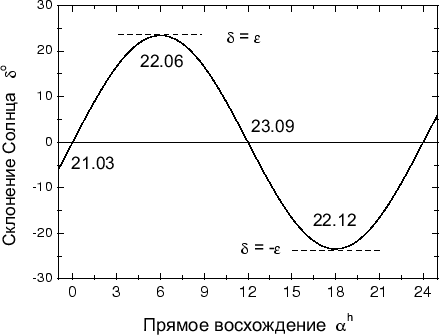
\includegraphics[width=0.6\textwidth]{change-coordin.png}
  \caption{График зависимости склонения от прямого восхождения Солнца}
 \end{figure}